\begin{figure*}[hbt!]
\centering
%%%%%%%%%%%%%%%%%%%%%%%%%%%%%%%%%%%%%
\begin{subfigure}[b]{.47\textwidth}
\begin{lstlisting}[basicstyle=\scriptsize\sffamily, stepnumber=1, numbers=left, numbersep=-8pt, framexleftmargin=-2mm, framexrightmargin=-2mm, emph ={allGames, game}]
    List<Game> allGames = gameMapper.getAllGamesByLeague(league);
    for (Game game : allGames) {
        game.getTeam1().setGame(game);
        game.getTeam2().setGame(game);
    }
    Collections.sort(allGames, new GameComparator());
\end{lstlisting}
%\caption{A listing}
\end{subfigure}
%%%%%%%%%%%%%%%%%%%%%%%%%%%%%%%%%%%%%%%%%%%%
\begin{subfigure}[b]{.4\textwidth}
\begin{lstlisting}[basicstyle=\scriptsize\sffamily, stepnumber=1, numbers=left, numbersep=-8pt, framexleftmargin=-2mm, framexrightmargin=-2mm, emph = {annotationVersion, annotation}]
    private boolean isValidUntil(Until annotation) {
        if (annotation != null) {
            double annotationVersion = annotation.value();
            if (annotationVersion <= version) {
                return false;
            }
        }
        return true;
    }
\end{lstlisting}
\end{subfigure}
%%%%%%%%%%%%%%%%%%%%%%%%%%%%%%%%%%%%%%%%%%%%
\begin{subfigure}[b]{0.42\textwidth}
  \centering
  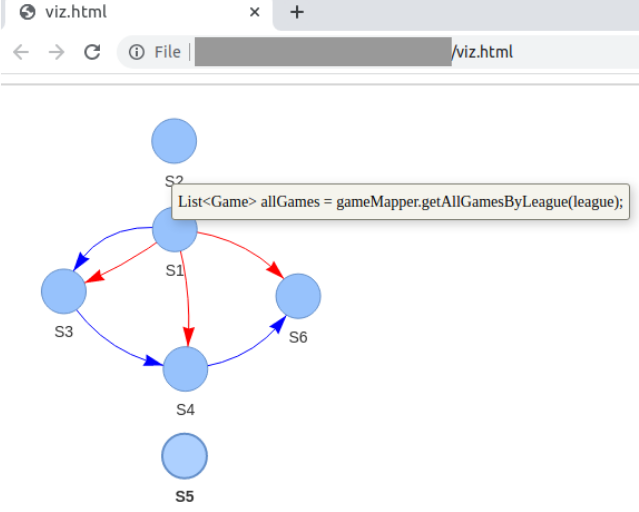
\includegraphics[width=0.7\linewidth]{icse23-demo-figures/lst-partial2.png}
  \vspace{0.75cm}
\end{subfigure}
%%%%%%%%%%%%%%%%%%%%%%%%%%%%%%%%%%%%%%%%%%%%
\begin{subfigure}[b]{.42\textwidth}
  \centering
  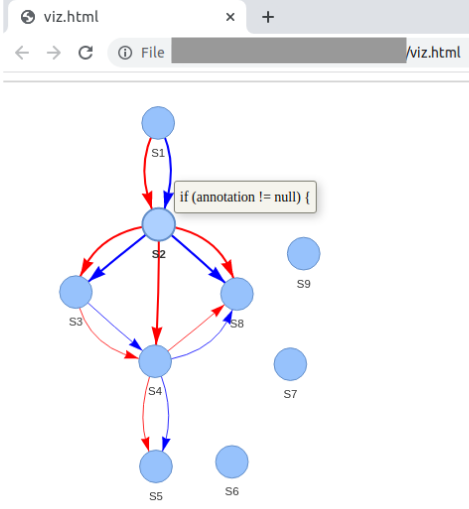
\includegraphics[width=0.7\linewidth]{icse23-demo-figures/lst-complete2.png}
\end{subfigure}
%%%%%%%%%%%%%%%%%%%%%%%%%%%%%%%%%%%%%%%%%%%%
\caption{Partial (top-left) and complete (top-right) Java code listings and their CFG/PDGs output by \tool (bottom).}
\label{fig:demo}
\vspace{-8pt}
\end{figure*}